{
\setbeamertemplate{background}{
\includegraphics[width=\paperwidth,height=\paperheight]{imagenes/fondo_simple.pdf}}

\begin{frame}{oFlute}
  \begin{columns}
    \column{0.6\textwidth}

    \begin{block}{}
      \begin{center}
        \Large
        Herramienta lúdico-educativa para el aprendizaje de la flauta dulce.

        \medskip
        \medskip

        Interacción del alumno con la flauta en tiempo real.
      \end{center}
    \end{block}

    \column{0.4\textwidth}
    \begin{block}{}
      \begin{center}
        \vspace{-1.5cm}
        
\includegraphics[width=0.6\textwidth]{imagenes/logotipo}

        \bigskip
        \bigskip

        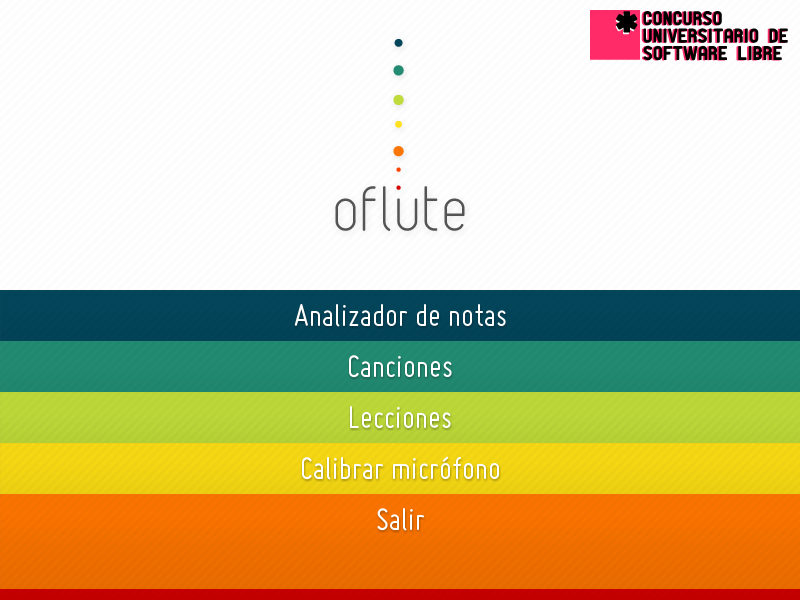
\includegraphics[width=\textwidth]{imagenes/imagen_menuPrincipal}
      \end{center}
    \end{block}   
  \end{columns}
\end{frame}


\begin{frame}{Analizador de notas}
  \begin{center}
    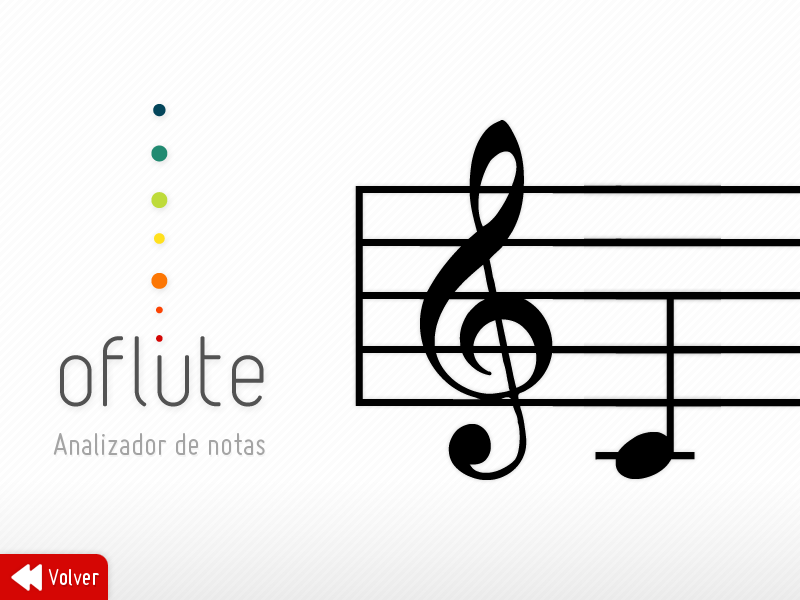
\includegraphics[width=0.7\textwidth]{imagenes/imagen_seccionAnalizador}

  Analiza las notas en tiempo real, de forma individual.
  \end{center}
\end{frame}

\begin{frame}{Motor de lecciones}

  \begin{center}
    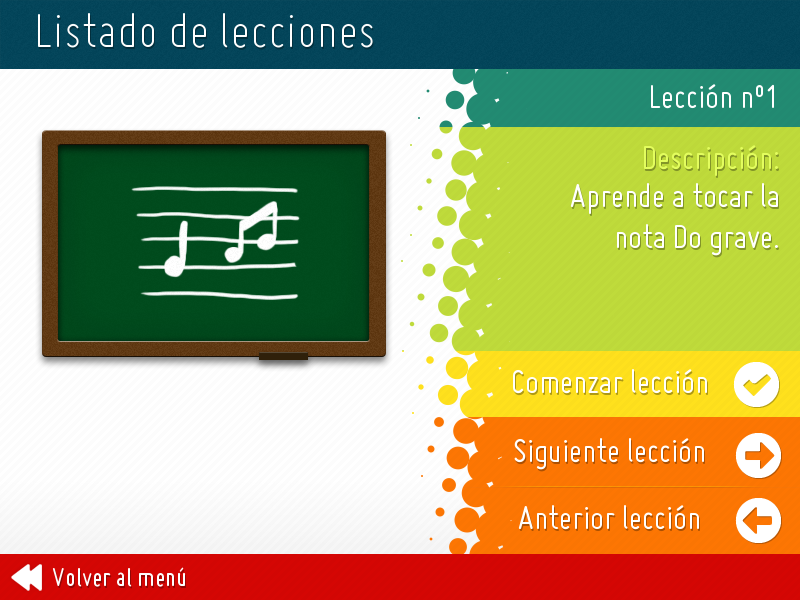
\includegraphics[width=0.49\textwidth]{imagenes/imagen_seccionLecciones1}\hspace{0.1cm}
    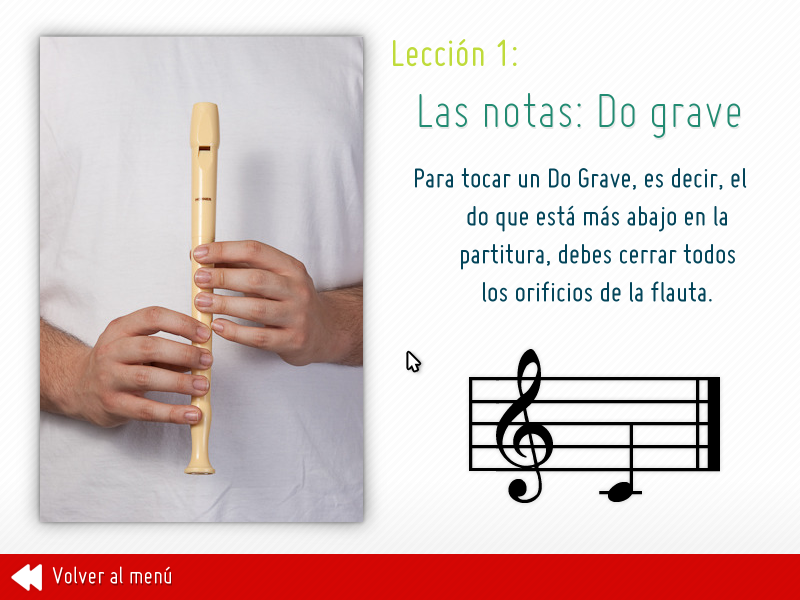
\includegraphics[width=0.49\textwidth]{imagenes/imagen_seccionLecciones2}

    \medskip

    Motor de lecciones con recursos multimedia, totalmente ampliable y personalizable.
  \end{center}

\end{frame}

\begin{frame}{Motor de canciones}

  \begin{center}
    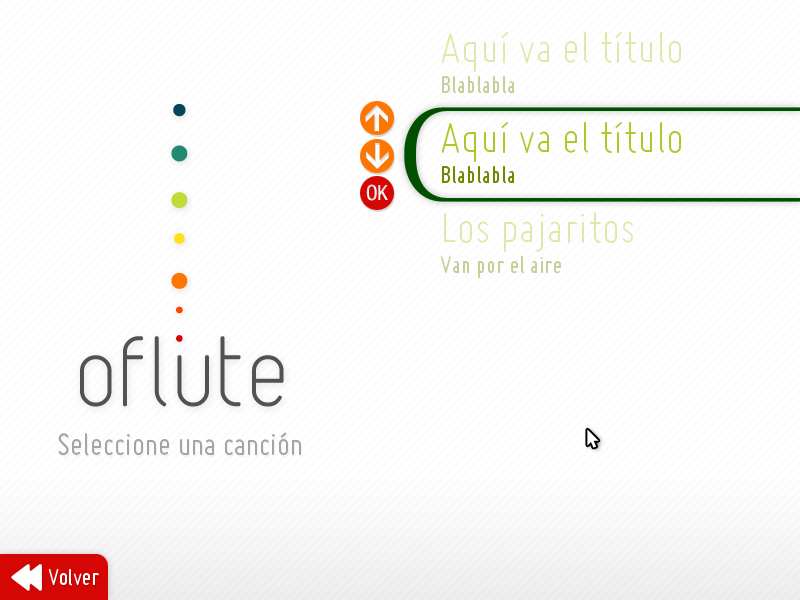
\includegraphics[width=0.49\textwidth]{imagenes/imagen_seccionCanciones1}\hspace{0.1cm}
    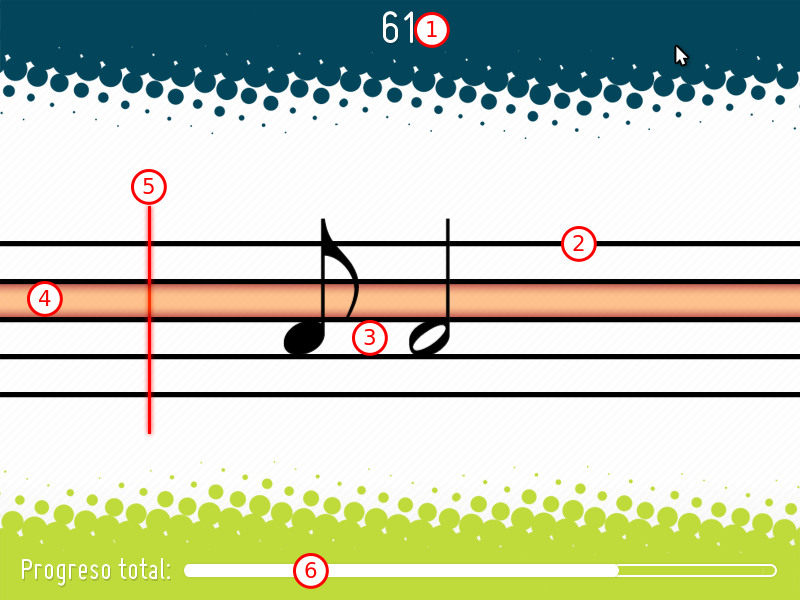
\includegraphics[width=0.49\textwidth]{imagenes/imagen_seccionCanciones2}

    \medskip

    Motor de canciones ampliable, permite la interpretación interactiva de canciones.
  \end{center}

\end{frame}
}

%%% Local Variables: 
%%% mode: latex
%%% TeX-master: "../presentacion"
%%% End: 
